\documentclass{../../text-style}

\texttitle{Лекция 10: Тестирование и дефекты}

\begin{document}

\maketitle
\thispagestyle{empty}

\section{Тестирование}

Зачем нужно тестирование, думаю, объяснять не надо, но есть шуточные аксиомы, которые любит упоминать Андрей Николаевич Терехов, и которые поясняют роль тестирования в разработке:

\begin{enumerate}
    \item Любая программа содержит ошибки.
    \item Если программа ошибок не содержит, их содержит алгоритм, который реализует программа.
    \item Если ни программа, ни алгоритм не содержат ошибок, эта программа даром никому не нужна.
\end{enumerate}

И правда, без ошибок можно написать разве что какой-нибудь Hello World, но он окажется даром никому не нужен. Все сколько-нибудь сложные и полезные системы ошибки неизбежно содержат, и задача процесса тестирования --- найти как можно больше из них, чтобы оставшиеся причиняли как можно меньше огорчений пользователям.

Напомним, что ошибки в программном обеспечении --- не несоответствие системы техническому заданию, а несоответствие системы ожиданиям пользователей, поэтому:

\begin{itemize}
    \item ошибки неизбежны просто потому, что у пользователей могут быть конфликтующие интересы --- желаемая функциональность для одного может быть критической ошибкой для другого;
    \item процесс тестирования субъективен --- тестировщик должен стараться поставить себя на место пользователя, а не слепо проверять следование спецификации.
\end{itemize}

Наверное, самое важное, что нужно понимать про тестирование --- это то, что тестирование не позволяет доказать, что ошибок в программе нет. Более того, попытка проверить всё заранее обречена на провал. Как писал Сэм Канер в своей знаменитой книге <<Тестирование программного обеспечения>>, <<Если вы убеждены, что можете полностью протестировать программу, не проверив её реакцию на каждую возможную комбинацию входных условий, --- прекрасно. Пришлите нам список предлагаемых вами тестов, и мы напишем программу, которая пройдёт их все и продемонстрирует эффектный сбой в пропущенной вами ситуации. Если мы сможем сделать это намеренно, то, без сомнений, подобная ошибка может быть допущена программистом и случайно>>\footnote{С. Канер и др., Тестирование программного обеспечения, Фундаментальные концепции менеджмента бизнес-приложений, Изд-во <<ДиаСофт>>, 2001. Цитата со стр. 42.}. Идея протестировать программу на всех входных данных заранее обречена на провал, потому что даже программа, складывающая два целых числа, имеет $2^{32^2}$ вариантов входных данных, и чтобы проверить их все, тратя, допустим, одну наносекунду на каждый, потребуется более 500 лет. А что будет, если числа вещественные?

Наверное, большинство из вариантов входных данных нам не интересно --- мы могли бы, зная как программа работает, разбить множество входных данных на подмножества, которые ведут себя одинаково. Кажется, в таком случае есть надежда всё-таки полностью проверить программу, и это на самом деле очень правильная идея, которая по-научному называется <<факторизация множества входных значений>>, тестировщики на самом деле этим занимаются постоянно. Но тут проблема в <<зная, как программа работает>> --- мы ведь ищем в программе ошибки, мы не можем быть уверены в том, что она работает так, как нам надо. Однако, имея исходники программы, мы, наверное, могли бы выделить такой набор входных данных, на которых все строки программы будут посещены --- но вдруг ошибка не в конкретной строке, а в комбинации условий, которые складывались в строках выше (например, в делении a на b нет ничего плохого, если b не 0, и у нас есть тест, где b не ноль, и тест, где b равно 0, но до деления программа не доходит).

Хорошо, мы тогда могли бы проверить все возможные пути исполнения, то есть все возможные комбинации исполняющихся строк кода, и тут-то быть уверенными, что программа работает правильно? Нет, не могли бы: опять-таки, в Канере описывается программа, написанная в 1979 году, состоящая из цикла и нескольких операторов if, для реализации которой в большинстве языков программирования потребовалось бы не больше 20 строк кода, однако эта программа имеет сто триллионов возможных путей исполнения. И ещё проблема, на которую Канер обращает внимание --- это что даже если вам вдруг удалось полностью протестировать программу (что бы это ни значило), надо будет тестировать её после каждого исправления или хотя бы перед каждым релизом новой версии.

Поэтому единственная задача процесса тестирования --- поиск ошибок. Из этого, кстати, следует, что если тест проблем не выявил --- он бесполезен и по сути пустая трата времени\footnote{Тут г-н Канер слишком категоричен, тесты ведь ещё и фиксируют корректную работу системы и если она когда-то будет нарушена, позволят об этом узнать --- это так называемые регрессионные тесты.}. Так что задача тестировщика --- придумать минимальный набор тестов, которые с максимальной вероятностью найдут ошибки в программе. Тут-то и помогает факторизация множества входных значений, знание о структуре и путях исполнения в программе, направленный фаззинг и другие приёмы. Но всё равно это творческая и неформализуемая работа, и всё равно, какими бы хорошими ни были тестировщики, ошибки в продукте всё равно будут. Наказывать тестировщиков за это нельзя, а вот поощрять за найденные ошибки можно.

Кстати, один из первых дефектов программного обеспечения был найден в 1947 году при работе с компьютером Harvard Mark II --- мотылёк попал между клеммами электромеханического реле и из-за него контакт не замыкался:

\begin{center}
    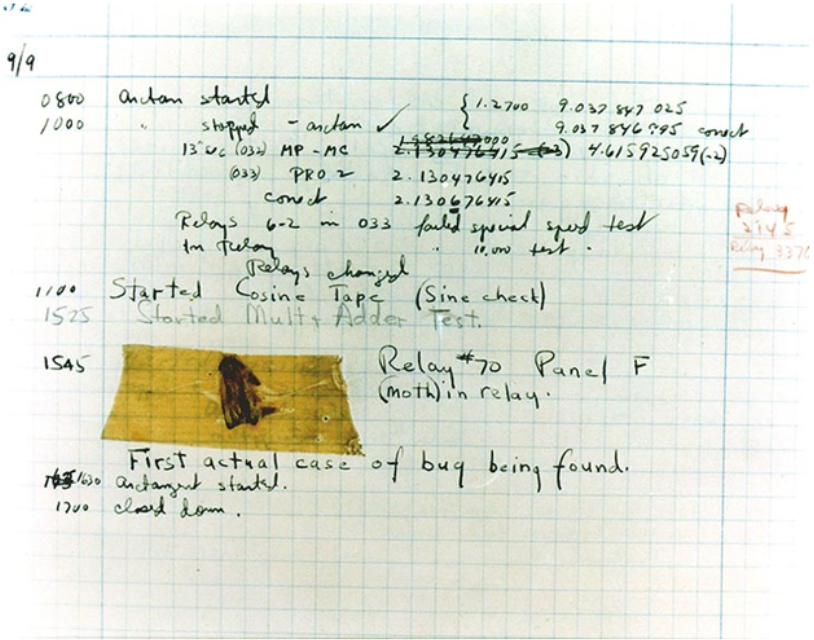
\includegraphics[width=0.8\textwidth]{bug.png}
    \attribution{https://education.nationalgeographic.org/resource/worlds-first-computer-bug/}
\end{center}

Однако, понятие <<bug>> в англоязычной литературе (или его нелепый перевод <<жучок>>) появилось задолго до этого инцидента --- ещё Эдисон в 1878 году называл дефекты в физических устройствах <<bug>> и говорил, что их надо очень долго выуживать до того, как продукт станет коммерчески успешным (можно обратить внимание, на рисунке иронично подписано <<first actual case of bug being found>>). Также обнаружение первого бага ошибочно приписывают известной учёному Грейс Хоппер, которая его на самом деле не нашла, но сделала знаменитым.

\subsection{Виды тестирования}

Поскольку тестирование --- это сложно, тестирование проводится по-разному и нацелено на поиск разных ошибок. Есть очень разная классификация видов тестирования, которая на практике не очень на самом деле полезна, но приводится здесь для обсуждения того, что и как в принципе можно тестировать.

Во-первых, классификация по тому, что именно тестируется.

\begin{itemize}
    \item Функциональное тестирование --- проверка работоспособности функциональности программы. Это то, что новички обычно подразумевают под тестированием вообще.
    \item Тестирование производительности --- проверка того, что система, даже если делает всё правильно, делает это за приемлемое время. Для систем реального времени или систем с жёсткими временными ограничениями, такими как, например, компьютерные игры, производительность может быть критичной. Но для <<обычных>> систем проблемы с производительностью также могут неожиданно приводить к резкому падению воспринимаемого пользователем качества (например, когда у веб-приложения внезапно растёт количество пользователей и оно перестаёт справляться с обработкой запросов). Тестирование производительности бывает:
    \begin{itemize}
        \item нагрузочным --- тестирование производительности под ожидаемой рабочей нагрузкой, с целью определить порог нагрузки, при переходе которого производительность становится слишком низкой;
        \item стресс-тестированием --- тестирование с нагрузкой, превышающей ожидаемую, чтобы посмотреть, как система себя поведёт (будет ли деградировать постепенно, или просто рухнет, оставив без обслуживания вообще всех пользователей);
        \item стабильности --- проверка работы под нагрузкой в течение длительного времени (например, чтобы выявить утечки памяти, неконтролируемый рост логов\footnote{Где-то, кажется, на \url{https://thedailywtf.com/} была история про систему, управляющую работой электронных замков в офисе, которая мирно проработала несколько лет и упала, когда все уже забыли, где она запущена, заполнив логами работы весь жёсткий диск и упав именно от того, что новый лог было писать некуда.} и другие проблемы, могущие возникнуть при длительной эксплуатации);
        \item конфигурации --- тестирование влияния конфигурационных параметров на производительность системы, начиная от базовых случаев типа опций компилятора, заканчивая конфигурацией балансировщиков нагрузки и кешей в распределённом приложении.
    \end{itemize}
    \item Тестирование пользовательского интерфейса --- проверка, что все кнопки и другие элементы управления на месте, кликабельны, и взаимодействие с ними приводит к ожидаемым эффектам.
    \item Тестирование удобства использования --- проверка, что приложение удобно и вызывает у пользователей положительные эмоции. Гораздо менее формально и гораздо менее автоматизируемо, чем перечисленные выше виды тестирования, но, пожалуй, даже более важно --- успех проектов определяется очень часто именно удобством использования, а не функциональностью или чем-либо ещё.
    \item Тестирование безопасности --- проверка защиты от навторизованного доступа и кражи данных/выполнения недопустимых операций. Ещё более безнадёжное дело, чем тестирование вообще, поскольку обеспечение безопасности --- это не просто поиск ошибки в коде, а игра против живого человека, как правило, мотивированного, умного и хорошо оснащённого. Поэтому цель любого обеспечения безопасности вообще --- не защита от взлома (\emph{любую} систему можно взломать), а обеспечение того, чтобы взлом был дороже потенциальной выгоды для взломщика. Тестирование безопасности, соответственно --- проверка не того, что систему нельзя взломать, а что её нельзя взломать \emph{просто}.
    \item Тестирование локализации --- проверка того, как выглядит пользовательский интерфейс при переключении на другой язык/локаль/культуру. Всё немного сложнее, чем кажется, поскольку локаль --- это не только перевод строк, это ещё и форматы чисел, дат, региональные особенности и буквально особенности культуры\footnote{Например, в китайском, японском и корейском языках иероглиф, обозначающий число <<четыре>>, созвучен в произношении с иероглифом, обозначающим <<смерть>>, так что будет очень плохой идеей присваивать пользователю идентификатор <<4>> в медицинском приложении. Сколько ещё таких культурных особенностей может быть среди пользователей вашего приложения, заранее сказать невозможно.}.
    \item Тестирование совместимости --- проверка того, что система работает на всех поддерживаемых аппаратных конфигурациях, операционных системах и в заданных окружениях. И что не мешает работать другим программам. Тоже, очевидно, крайне непростая задача просто исходя из возможного количества вариантов, плюс может быть ресурсозатратной, если требуется покупать экзотическое аппаратное обеспечение (пишете шутер --- извольте купить весь модельный ряд видеокарт всех ключевых производителей, да ещё и несколько популярных процессоров, потому что с ними тоже бывают странные проблемы).
\end{itemize}

По масштабности тестирования оно традиционно разделяется на:

\begin{itemize}
    \item модульное --- тестирование отдельных классов и методов, отдельных функций; как правило, осуществляется самими разработчиками;
    \item интеграционное --- тестирование взаимодействия двух или более модулей или более крупных компонентов системы; как правило, автоматизированное, и, как правило, выполняется специальными людьми --- автоматизаторами тестирования, поскольку требует написания большого количества кода для настройки/деинициализации тестового окружения и запуска самого тестового сценария;
    \item системное (в английской литературе <<end-to-end-тестирование>>) --- проверка пользовательских сценариев, начиная от пользовательского интерфейса; может быть автоматическим и ручным, также обычно выполняется выделенными для этого людьми (тестировщиками, включая автоматизаторов).
\end{itemize}

Обратите внимание, что только системным тестированием и даже интеграционным тестированием не обойтись --- возможных путей исполнения во всей программе так много, что нет ни единого шанса <<дёргая>> только пользовательский интерфейс или публичный интерфейс компонентов проверить сколько-нибудь значимый процент этих путей. Однако и модульного тестирования недостаточно:

\begin{center}
    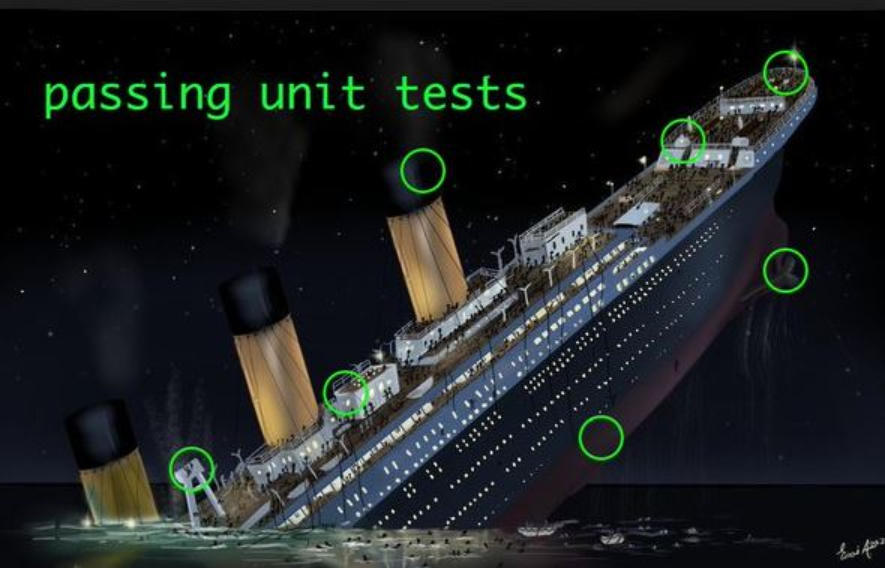
\includegraphics[width=0.6\textwidth]{titanic.png}
    \attribution{https://blogs.sap.com/2018/04/21/sap-open-course-unit-testing-week-6-working-with-existing-code/}
\end{center}

Также бывает классификация по этапу жизненного цикла.

\begin{itemize}
    \item <<Смоук-тестирование>> (англ. smoke testing) --- тестирование при передаче новой функциональности тестировщикам. Есть две версии появления этого названия --- правильная: от инженеров-электронщиков, включаем прибор в розетку, если он задымился, тестировать его дальше смысла нет; и поясняющая суть дела --- тест, который можно успеть закончить до того, как тестировщик докурит сигарету. Тестируется основной сценарий, чтобы убедиться, что система вообще хоть как-то работает, и если смоук-тест не прошёл, систему сразу возвращают на доработку (интересно, что в реальности некоторые программисты не утруждают себя даже собрать написанный ими код, так что смоук-тесты необходимы и очень актуальны).
    \item Регрессионное тестирование --- проверка после изменений в системе, что старые ошибки не начали вновь проявляться. Модульное тестирование регрессионно по своей сути, поскольку единожды написанный модульный тест, как правило, остаётся в системе навсегда и запускается после каждой сборки (или хотя бы перед каждым релизом). Но ручное регрессионное тестирование также часто необходимо.
    \item Альфа-тестирование --- тестирование ещё не законченного продукта, в котором, однако, большая часть функциональности уже реализована и в целом он работоспособен. Часто проводится всей командой разработчиков (например, <<playtesting>> при разработке игр). Однако при альфа-тестировании вовне продукт обычно не отдают, в отличие от бета-тестирования. Важное исключение --- программы типа <<early access>> в Steam, где пользователи могут следить за разработкой и выполнять альфа-тестирование, купив продукт обычно за меньшие деньги, чем после релиза.
    \item Бета-тестирование --- тестирование реальными пользователями. На бета-тест выставляется обычно уже готовый продукт, при этом бета-тестирование бывает открытым и закрытым. Закрытое бета-тестирование предполагает тестирование ограниченным кругом специально приглашённых пользователей, открытое --- кем угодно. Закрытое позволяет минимизировать репутационные потери от низкого качества продукта, однако открытое позволяет задействовать больше пользователей и найти больше ошибок. Некоторые продукты живут в стадии бета-тестирования годами и вполне коммерчески успешны.
    \item Релиз-кандидат --- версия системы, которая считается разработчиком законченной достаточно качественной для тестирования, однако требует полной проверки со стороны тестировщиков и, зачастую, пользователей, участвующих в бета-тестировании, прежде чем стать релизом. По мере исправления выявленных ошибок могут появляться следующие версии релиз-кандидатов.
\end{itemize}

Также может быть полезна классификация по уровню знаний о тестируемой системе:

\begin{itemize}
    \item Тестирование <<чёрного ящика>> --- когда проверяется только взаимодействие системы и внешнего мира, устройство системы считается неизвестным.
    \item Тестирование <<белого ящика>> --- когда тестировщик имеет полный доступ к исходным кодам системы и может использовать информацию о её внутреннем устройстве для направленного тестирования.
    \item Тестирование <<серого ящика>> --- когда тестировщик имеет доступ к некоторой информации о системе или имеет возможность измерять некоторые её внутренние параметры, которые обычно не видны наружу. Например, фаззинг, генерирующий случайные входы, может использовать информацию о покрытии строк исходного кода, чтобы это покрытие целенаправленно максимизировать.
\end{itemize}

Кажется, что тестировщики всегда имеют доступ к исходному коду, и тестирование белого ящика лучше, поскольку позволяет задействовать больше информации, поэтому тестирование чёрного ящика не нужно. Однако на практике тестирование чёрного ящика используется чаще, и зачастую полезнее --- этот подход позволяет взглянуть на систему глазами пользователя, которому нет дела до внутреннего устройства системы, и сосредоточиться на внешних свойствах системы, а не на максимизации тестового покрытия или корректности архитектуры.

Ещё тестирование бывает исследовательским --- когда тестировщик исследует систему, пытаясь выяснить, что она уже умеет, и вообще знакомится с системой. Исследовательское тестирование, как правило, тоже не просто <<потыкался>>, а более структурное (как минимум, ведётся съёмка экрана/логирование действий, чтобы если вдруг встретится ошибка, её можно было легко задокументировать).

\section{Тестирование и жизненный цикл}

Тестирование в обывательском представлении --- это когда система уже готова и тестировщик садится искать в ней ошибки. Это, конечно же, не так --- если система уже готова и тестировщик видит её в первый раз, тестировать её уже поздно. Работа тестировщика начинается ещё в самом начале проекта, на этапе сбора требований, и не заканчивается до вывода продукта из эксплуатации.

\subsection{Тестирование требований}

Начинается всё с тестирования требований. Хорошие требования составляются с участием тест-лида, который контролирует, что требования вообще проверяемы, но иногда бывает, что команде приносят уже готовую SRS\footnote{Software Requirement Specification, документ, обсуждавшихся на одной из первых лекций курса.}. В этом случае тестировщики должны проверить адекватность требований.

Ничего формального и тем более автоматизируемого индустрия для этого не придумала (по крайней мере, активно не применяет). Большая часть тестирования требований сводится к экспертной оценке и дискуссиям внутри команды. Основная цель таких обсуждений --- выявление скрытых неоднозначностей\footnote{Хороший пример --- two zero two four --- это 2024, 0044, 2044, 0024?}, побочный эффект --- распространение знаний и общего видения требований внутри команды. Наиболее продуктивны такие мероприятия, если в них участвуют помимо тестировщиков разработчики и представители бизнеса --- последние представляют интересы клиента, разработчики должны понимать, что от них хотят, тестировщики должны понимать, как именно это проверять (определить то, что называется <<критерии приёмки>>, <<acceptance criteria>>). 

Поговорим подробнее, что и как надо проверять в требованиях.

\begin{itemize}
    \item Однозначность --- это самое важное:
    \begin{itemize}
        \item в основном, путём дискуссий, как описано выше;
        \item следить за словами <<обычно>>, <<как правило>>, <<иногда>>, <<необязательно>> и т.п.;
        \item следить за субъективными оценочными суждениями: <<удобно>>, <<быстро>>, <<гибко>> и т.п.
    \end{itemize}
    \item Отсутствие соединительных предлогов (<<и>>, <<или>>) --- они указывают на неатомарность требований, что нехорошо.
    \item Наличие чёткого критерия приёмки --- когда требование считается реализованным.
    \item Отсутствие избыточных и противоречивых требований. Избыточных не в том смысле, что пользователю это не надо, а в том, что одно требование полностью покрывает другое.
    \item Понимание, для кого это требование, все ли роли, заинтересованные в реализации этого требования, учтены, мотивация каждой роли.
    \begin{itemize}
        \item Ещё надо проверить, что описание требования не предполагает конкретного способа реализации --- иначе к его описанию, скорее всего, приложили руку программисты.
    \end{itemize}
\end{itemize}

Вообще, в принципе, чтобы требование стало требованием и попало в бэклог (или просто стало задачей для разработки), его можно проверить на соответствие критериям INVEST (требования суть менеджерская штука, менеджеры любят звучные аббревиатуры):

\begin{itemize}
    \item I --- Independent, независимое от остальных;
    \item N --- Negotiable, то есть его можно обсудить и изменить\footnote{Кажется, оно тут только для того, чтобы IVEST не получилось, но кто мы такие, чтобы спорить...};
    \item V --- Valuable, имеющее ценность для пользователя;
    \item E --- Estimable, трудоёмкость его реализации можно оценить;
    \item S --- Small, его можно реализовать в разумные сроки (один спринт или одну итерацию разработки, иначе надо декомпозировать);
    \item T --- Testable, можно протестировать его выполнение.
\end{itemize}

Каждому требованию должны соответствовать критерии приёмки, одно или больше. При этом хорошие критерии приёмки должны быть предельно чёткими, в форме <<контекст $\to$ действие>>, то есть <<находясь в таком-то состоянии работы с системой пользователь может сделать то-то>>. Критерии приёмки должны однозначно документировать поведение системы в рассмотренных ситуациях. Ещё критерии приёмки часто включают в техническое задание, поэтому у неопытных разработчиков возникает естественное желание сделать их как можно более обтекаемыми и простыми в реализации --- этого делать нельзя, критерии приёмки должны быть добросовестными. <<Втюхать>> заказчику некачественный продукт, конечно, можно, но репутационные потери от этого в большинстве случаев легко перевесят плюсы от закрытого договора. Если вы не хотите, чтобы этот проект оказался для вас последним, критерии приёмки должны покрывать все интересные заказчику требования и быть действительно годным планом тестирования, заранее согласованным с заказчиком, командой разработчиков и службой контроля качества.

\subsection{Тестирование архитектуры}

Тестирование архитектуры тоже процесс слабоформализуемый и проходящий в виде совместного анализа архитектуры. При этом следует обращать внимание на следующие важные для тестируемости продукта вещи.

\begin{itemize}
    \item Аккуратность декомпозиции системы. Клубок из хаотично вызывающих друг друга классов или компонентов протестировать невозможно, потому что невозможно (или стоит больших усилий) выделить отдельный модуль для тестирования и изолировать его от остальных. Архитектура должна позволять легко подменять модули на тестовые заглушки (<<Mock>>-и), для этого должны активно применяться принципы инверсии зависимостей (Dependency Inversion), аккуратное разделение на слои. Для распределённых приложений помогает микросервисная архитектура, но её наивное применение может привести к <<микросервисному монолиту>>, где каждый микросервис дёргает каждый, и это тестировать ещё сложнее.
    \item Простота. Сложную систему тестировать сложнее, поэтому <<архитектурное астронавтство>>, когда задача решается существенно более сложным способом, чем могла бы, должно вызывать соответствующую реакцию тестировщика. Обычно так происходит из благих побуждений --- <<вот это у нас задел на будущее>>, <<это обеспечивает гибкость>> и т.п. Однако как правило, усложнение архитектуры в надежде в будущем упростить разработку совершенно не окупается, а проблемы создаёт уже сейчас. Плюс к тому, практика показывает, что лучший способ упростить разработку в будущем --- сделать максимально простую архитектуру сегодня, чтобы в будущем было легко с ней разобраться и её модифицировать.
    \item Пожалуй, самое важное --- наблюдаемость. С  ним есть две проблемы --- тестировщик не получает никакой информации о состоянии системы и не может делать выводы, что с ней происходит, и тестировщик получает слишком много информации о состоянии системы и не может делать выводы, что с ней происходит. Поэтому хорошая архитектура должна учитывать:
    \begin{itemize}
        \item возможность развернуть систему и окружение специально для тестирования;
        \item быстроту обратной связи --- тестировщику должно быть не нужно долго ждать при воспроизведении тестового сценария (тут всё зависит не только от архитектуры, но и от автоматизации тестирования, но плохая архитектура делает это невозможным);
        \item логирование --- по логам должно быть быстро понятно, что и где упало, поэтому используются структурные логи (не текст, а JSON-документы, например) и системы управления логами, типа ElasticSearch и Kibana;
        \item трассируемость --- в распределённой системе логировать действия недостаточно, потому что логи ведёт каждый компонент системы отдельно, а как один запрос пользователя обрабатывается разными компонентами, без ухищрений типа идентификаторов корреляции невозможно;
        \item метрики, метрики, метрики --- отслеживание в реальном времени различных параметров состояния системы, от потребляемой памяти до количества продаж в магазине (то, что называется <<конверсий>>) в секунду; опять-таки, метрики должны быть структурированы, централизовано собираться и визуализироваться (Grafana).
    \end{itemize}
\end{itemize}

\subsection{Тестирование и реализация}

Теперь поговорим о том, как тестирование выполняется в процессе реализации, контроля качества и выпуска продукта. Обратите внимание, в современных методологиях разработки тестирование обычно не выносится в отдельную фазу, а выполняется параллельно с разработкой.

\subsubsection{Пирамида тестирования}

Как мы знаем, тесты бывают модульными, интеграционными и системными, и все они необходимы. Разработка модульных тестов проще всего и работают они быстрее остальных тестов, а системное тестирование (включая тестирование пользовательского интерфейса) --- наоборот, наиболее трудоёмкий и медленный процесс (зачастую требующий ручного тестирования), поэтому, естественно, модульных тестов в проекте больше. Это соображение известно в индустрии как <<пирамида тестирования>>:

\begin{center}
    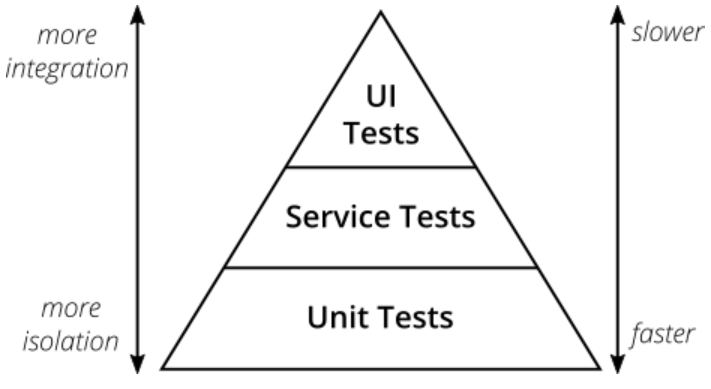
\includegraphics[width=0.6\textwidth]{testPyramid.png}
    \attribution{https://martinfowler.com/articles/practical-test-pyramid.html}
\end{center}

Модульные тесты пишутся всегда и для всего, и запускаются всегда, при каждом коммите в систему контроля версий (делают это системы непрерывной интеграции). При этом собирается информация об исполненных в ходе тестового прогона строках, и считается приличным поддерживать покрытие строк кода в районе 90-100\%. Остаются непротестированными обычно редкие сценарии возникновения ошибок, которые требуют очень сложных манипуляций для приведения системы в ошибочное состояние --- не потому что их не надо тестировать, а потому что времени не хватает. Тестировать ошибочные сценарии как раз очень надо, некорректное поведение при обработке ошибок встречается в системах гораздо чаще, чем при <<хороших>> сценариях --- программисты хотят, чтобы работало, а не чтобы правильно реагировало на некорректный ввод или отказы оборудования.

Интеграционные тесты (то, что у Фаулера называется <<Service tests>>) работают дольше и запускаются обычно реже, например, каждой ночью. И писать их дольше и сложнее, поэтому в проекте обычно их меньше, чем модульных.

Системные тесты и тесты пользовательского интерфейса тоже запускаются не каждый коммит (хотя зависит, короткие UI-тесты вполне допустимо включать в непрерывную интеграцию), и часто требуют ручной проверки. Даже если все сценарии можно автоматизировать, нередки случаи, когда с программной точки зрения всё ок, но человек, вручную прогнав тестовый сценарий, сразу заметит ошибку (например, чёрная кнопка на чёрном фоне --- автоматика кликнет по координатам без проблем, людям не понравится).

\subsubsection{Тестовые сценарии}

Для ручного тестирования и зачастую для автоматизации тестирования тоже описывают формально набор тестовых сценариев (или, часто, тест-кейсов) --- что надо проверять, какие действия совершать и что должно получиться. Тестовые сценарии бывают неформальными, когда просто текстом на естественном языке описывается, что надо проверить, бывают более структурированными, состоящими из:

\begin{itemize}
    \item идентификатора и названия --- чтобы на сценарий было можно ссылаться, и чтобы было понятно, о чём он;
    \item набора предварительных шагов по подготовке тестируемой системы (<<System Under Test>>, <<SUT>>);
    \item набора шагов, собственно тестирующих систему --- каждый шаг состоит из пары <<действие --- ожидаемый результат>>;
    \item итоговый ожидаемый результат --- что мы должны наблюдать после исполнения всего сценария;
    \item дополнительно могут быть описаны шаги по восстановлению окружения после теста, если это нетривиально (откатить изменения в базе данных, например).
\end{itemize}

Помимо этого у тестовых сценариев может быть:

\begin{itemize}
    \item конфигурация --- набор параметров окружения, в котором выполняется сценарий; при реальном прогоне выбирается конкретное множество параметров, что превращает один сценарий в потенциально очень много отдельных конкретных сценариев (например, проверить на трёх разных ОС и на пяти разных браузерах на каждой ОС);
    \item набор тэгов, нужных для структурирования множества тестовых сценариев;
    \item набор зависимостей --- какие сценарии нужно прогнать до/после, при изменении в какой части кода надо перепроверить сценарий.
\end{itemize}

Тестовые сценарии объединяются в сьюты (от англ. <<suite>>) --- наборы сценариев, которые обычно требуется прогонять вместе. также сценарии могут быть сгруппированы в проекты (ортогонально сьютам), по их отношению к разрабатываемым компонентам системы. Для чего нужны тэги, сьюты и проекты, будет понятно, если учесть, что в реальной жизни количество тестовых сценариев измеряется тысячами для типичных проектов, и без средств группировки и удобного поиска и классификации управлять ими очень сложно.

Помимо тестовых сценариев, есть ещё тестовые прогоны --- можно сказать, экземпляры сценариев, когда тестировщик, вручную или автоматически, исполнил сценарий и записал результат. У прогона есть дата прохождения, статус (успешно, с ошибкой, пока не пройден, заблокирован известной ошибкой и т.п.), иногда статус по каждому шагу. 

Прогоны объединяются в тест-планы --- это отобранные тестовые сценарии для проверки той или иной функциональности. Ведущий тестировщик отбирает из сьют и проектов тестовые сценарии, создаёт (автоматически, в системе управления тестами) тестовые прогоны в статусе <<запланирован>>, назначает на них тестировщиков, назначает календарные даты (привязанные к датам релизов продукта и исходя из объёмов тестирования). Дальше прогоны исполняются, результаты заносятся в трекер ошибок, если ошибки выявлены, и в систему управления тестированием в любом случае, и когда тестовый план исполнен, отдел контроля качества даёт отмашку на релиз.

\subsubsection{Пример тестового сценария}

Вот небольшой пример тестового сценария из книги Канера\footnote{С. Канер и др., Тестирование программного обеспечения, Фундаментальные концепции менеджмента бизнес-приложений, Изд-во <<ДиаСофт>>, 2001.}: хочется написать программу, складывающую два двузначных числа. 

Сначала смоук-тестирование, на работоспособность программы в самом частом сценарии её использования: 

\begin{center}
    \begin{tabu} {| X[0.6 l p] | X[1 l p] |}
        \tabucline-
        \everyrow{\tabucline-}
        \textbf{Что делаем}                             & \textbf{Что происходит}                                                            \\
        Вводим \textit{adder} и жмём на \textit{Enter}  & Экран мигает, внизу появляется знак вопроса                                        \\
        Нажимаем 2                                      & За знаком вопроса появляется цифра 2                                               \\
        Нажимаем \textit{Enter}                         & В следующей строке появляется знак вопроса                                         \\
        Нажимаем 3                                      & За вторым знаком вопроса появляется цифра 3                                        \\
        Нажимаем \textit{Enter}                         & В третьей строке появляется 5, несколькими строками ниже --- ещё один знак вопроса
    \end{tabu}
\end{center}

Вот это и есть тестовый сценарий. Обратите внимание, он составлен так, что в нём чётко прописано каждое действие тестировщика и отдельно чётко прописан ожидаемый результат. Задача простая, вряд ли разработчик мог ошибиться в такой программе, однако хороший тестировщик после смоук-теста уже выявил бы три проблемы.

\begin{itemize}
    \item Нет названия программы на экране, может, мы запустили не то
    \item Нет никаких инструкций, пользователь без идей, что делать. Программа просто показывает чёрный экран и мигает курсором.
    \item Непонятно, как выйти.
\end{itemize}

Понятно, что ни одна из этих ошибок с точки зрения требований ошибкой не является, но тестировщик выявил потенциальные проблемы со стороны пользователя, а не несоответствие ТЗ.

Теперь надо проверить поведение программы на разных входных данных, поэтому придумаем ещё один тестовый сценарий. Стараемся <<на глаз>> кластеризовать множество входных данных так, чтобы покрыть подозрительные варианты, и выбираем из каждого кластера наиболее интересный представитель:

\begin{center}
    \begin{tabu} {| X[2 l p] | X[2 l p] | X[7 l p] |}
        \tabucline-
        \everyrow{\tabucline-}
        \textbf{Ввод}  & \textbf{Ожидаемый результат}  & \textbf{Замечания}                                                      \\
        99 + 99        & 198                           & Пара наибольших допустимых чисел                                        \\
        -99 + -99      & -198                          & Отрицательные числа, почему нет?                                        \\
        99 + -14       & 85                            & Большое первое число может влиять на интерпретацию второго              \\
        -38 + 99       & 61                            & Отрицательное плюс положительное                                        \\
        56 + 99        & 155                           & Большое второе число может повлиять на интерпретацию первого            \\
        9 + 9          & 18                            & Два наибольших числа из одной цифры                                     \\
        0 + 0          & 0                             & Программы часто не работают на нулях                                    \\
        0 + 23         & 23                            & 0 --- подозрительная штука, его надо проверить и как первое слагаемое,  \\
        -78 + 0        & -78                           & и как второе
    \end{tabu}
\end{center}

Ну и, конечно, проверка некорректного ввода, ещё один сценарий:

\begin{center}
    \begin{tabu} {| X[2 l p] | X[7 l p] |}
        \tabucline-
        \everyrow{\tabucline-}
        \textbf{Ввод}                   & \textbf{Замечания}                                                 \\
        100 + 100                       & Поведение сразу за диапазоном допустимых значений                  \\
        \textit{Enter} + \textit{Enter} & Что будет, если данные не вводить вообще                           \\
        123456 + 0                      & Введём побольше цифр                                               \\
        1.2 + 5                         & Вещественные числа, пользователь может решить, что так можно       \\
        A + b                           & Недопустимые символы, что будет?                                   \\
        Ctrl-A, Ctrl-D, F1, Esc         & Управляющие клавиши часто источник проблем в консольных программах \\
    \end{tabu}
\end{center}

Но и это ещё не всё. Зная, как примерно могла бы быть реализована такая программа, хороший тестировщик проверит тестовые случаи, опасные для конкретной реализации.

\begin{itemize}
    \item Внутреннее хранение данных --- двузначные числа есть большой соблазн хранить в \textbf{byte}, от -128 до 127, но тогда результат сложения может вызывать переполнение, надо это проверить.
    \begin{itemize}
        \item 99 + 99, этот случай покрыли.
    \end{itemize}
    \item Кодовая страница ввода: символы '/' и '0', '9' и ':' находятся там рядом, поэтому программист может напутать со строгостью неравенства при проверке того, цифра введённый символ или нет.
    \begin{itemize}
        \item Можно упростить тесты: не надо вводить A + b, достаточно граничные символы.
    \end{itemize}
\end{itemize}

\subsection{Инструменты тестирования}

Теперь немного поговорим об инструментах тестировщика. Хорошая новость в том, что большую часть работы можно делать не вручную.

\subsubsection{Модульное тестирование}

Для модульного тестирования существуют, во-первых, библиотеки модульного тестирования.

\begin{itemize}
    \item JUnit и его многочисленные идейные продолжатели в разных языках (например, NUnit для .NET, pytest для Python) --- описываем тест в виде трёх фаз:
    \begin{itemize}
        \item инициализации тестового окружения (System Under Test, SUT);
        \item выполнения действия над SUT;
        \item проверки результатов в виде серии вызовов методов класса Assert.
    \end{itemize}
    \item Библиотеки \emph{матчеров}, такие как Hamcrest или NHamcrest, позволяющие вместо \mintinline{csharp}{Assert.AreEqual(1, f())} писать \mintinline{csharp}{Assert.That(f(), Is.EqualTo(1))} и комбинировать по-всякому логические условия, что должно сделать тест более читаемым.
    \item Библиотеки тестирования, основанного на свойствах, такие как QuickCheck/FsCheck --- где мы проверяем систему не на конкретных данных, а выписываем предикат, которому система должна всегда удовлетворять, и библиотека забрасывает систему случайно сгенерированными данными, проверяя на каждом наборе данных выполнимость предиката. Работает это на самом деле неплохо, современные библиотеки даже могут сами построить минимальный пример, где предикат нарушается.
    \item Библиотеки символьного исполнения, которые вообще не гоняют тесты на данных, а пытаются статически вывести, насколько это возможно, корректность тестируемого кода, анализируя диапазоны значений входных данных (автор видел в реальной практике только одну такую библиотеку --- Unquote, но с совершенствованием решателей и символьных интерпретаторов этот подход, кажется, становится всё более популярен).
\end{itemize}

Во-вторых, важны библиотеки для генерации тестовых заглушек, такие как Mockito, Moq и много-много других. Тестовая заглушка --- код, который ведёт себя как настоящий класс/компонент, но на самом деле ничего не делает, а просто возвращает значения, которые ему сказали, и записывает все вызовы своих методов, чтобы их можно было проверить. Заглушки подставляются в System Under Test при её инициализации вместо реальных зависимостей, настраиваются на конкретный тестовый сценарий, и проверяется, что SUT ведёт себя, как положено. Выглядит это, например, так (библиотека Mockito, Java, пример из документации\footnote{Домашняя страница Mockito, URL: \url{https://site.mockito.org/} (дата обращения: 24.04.2023)}):

\begin{minted}{java}
LinkedList mockedList = mock(LinkedList.class);
// or even simpler with Mockito 4.10.0+
// LinkedList mockedList = mock();

// stubbing appears before the actual execution
when(mockedList.get(0)).thenReturn("first");

// the following prints "first"
System.out.println(mockedList.get(0));

// the following prints "null" because get(999) was not stubbed
System.out.println(mockedList.get(999));
\end{minted}

Соответственно, этот список мы можем передать любому классу, который ожидает список как зависимость (например, принимает в конструктор), и проверить, что он реально вызывает get. Объекты-заглушки в тестах часто кладут в IoC\footnote{Inversion of Control-контейнеры, библиотеки для управления зависимостями и инициализации объектов (например, Spring IoC).}-контейнеры, чтобы SUT автоматически инициализировалась именно ими.

\subsubsection{Тестирование интерфейсов}

Для тестирования пользовательских интерфейсов применяют программы-драйверы, генерирующие события пользовательского интерфейса. Безусловным лидером в таких системах является Selenium, который умеет управлять браузерами и симулировать как реальные клики, так и непосредственно работать с Document Object Model страницы в браузере. Последнее, помимо того, что делает написание теста более удобным (<<кликни на кнопку с id таким-то>>, а не <<кликни по таким-то координатам, ой, подожди, вёрстку страницы вчера поменяли>>), позволяет использовать <<безголовый>> режим работы браузера (то есть без пользовательского интерфейса, только DOM + JavaScript), что позволяет тестировать пользовательские интерфейсы на сервере непрерывной интеграции, где выводить пользовательский интерфейс некуда. Selenium умеет искать элементы страницы по CSS или XPath-запросам, но для удобства тестирования надо придерживаться правила, что у каждого элемента страницы должен быть уникальный идентификатор, желательно осмысленный для человека, не автогенерённый.

Для тестирования десктопных приложений тоже есть инструменты, например, White для тестирования .NET-приложений (вообще, их много разных). Тестирование десктопных приложений требует поддержки со стороны операционной системы (например, Windows Accessibility API).

Для тестирования программных интерфейсов, например, веб-API, используют специализированные исполнители запросов, такие как Postman (отладочные прокси типа Fiddler тоже умеют исполнять и модифицировать тестовые запросы, но не так удобно). Ещё очень полезны инструменты фаззинга веб-приложений (которые просто бомбардируют сайт случайными запросами, часто даже с нарушением низкоуровневых протоколов, чтобы посмотреть, как сайт себя поведёт) и автоматического поиска уязвимостей безопасности (конкретных примеров ни фаззеров, ни сканеров безопасности не приведу, не работал с такими штуками).

\subsubsection{Системы управления тестированием}

Наконец, немного про системы, куда писать тестовые сценарии, прогоны и результаты.

\begin{itemize}
    \item Электронная почта, электронные таблицы, онлайн текстовые редакторы и т.п. --- работает для небольших проектов, однако в общем случае очень плохая идея, потому что неизбежна путаница, кто что проверил, кто что должен проверять, что поправлено и т.п., особенно с учётом того, что тестовых сценариев тысячи. У коллег был опыт использования интеллект-карт (mind maps) для неформального описания тестовых сценариев, опыт скорее негативный.
    \item TestRail --- очень популярная в индустрии система, умеет делать всё, что должны уметь подобного рода системы (то есть тестовые сценарии, прогоны, сьюты, тест-планы и т.д.). Но старенькая, аж 2004 года, хоть и активно развивается.
    \item Test IT, Xray, Kiwi TCMS и т.д., последняя с открытым исходным кодом, однако много чего не умеет. Есть ещё Sitechko, учебная система, в которой можно поиграться с этими делами, и она довольно неплоха, но в реальных проектах вроде не используется.
    \item TestY, система, разрабатываемая с активным участием студентов матмеха, тоже с открытым исходным кодом, и тоже пока умеет не всё, но есть перспективы.
\end{itemize}

Тестовые сценарии, разумеется, могут быть автоматизированы, поэтому хорошие системы управления тестированием должны уметь интегрироваться с библиотеками модульного тестирования, чтобы отображать статус модульных тестов.

\section{Отслеживание ошибок}

Положим, наши тестовые прогоны выявили ошибки, и надо что-то с этим делать. Пойти и жаловаться на жизнь разработчику в надежде, что он что-то поправит, плохая идея (хотя в том же Канере описывается, как они в 1980-х клали разработчикам на стол пачку бумажных сообщений об ошибках и требовали под каждым подписи разработчика, что он ознакомлен). Надо, чтобы каждая ошибка учитывалась в планировании, ни про одну не забыли, в конечном итоге все (ну, не обязательно, но в идеале) были исправлены. Поэтому в команде должен быть налажен процесс отслеживания ошибок.

\subsection{Основные атрибуты сообщения об ошибке}

Начинаться всё должно с корректного описания ошибки. Грамотное сообщение должно состоять из следующих вещей.

\begin{itemize}
    \item Уникальный идентификатор ошибки, по которому не неё легко ссылаться.
    \item Заголовок, кратко, но ёмко описывающий суть проблемы.
    \item Описание дефекта, самая важная часть сообщения об ошибке:
    \begin{itemize}
        \item контекст, в котором возникла ошибка, включая, обязательно, версию системы, параметры окружения;
        \item шаги воспроизведения --- минимальный, воспроизводимый и понятный разработчикам набор действий, приводящих к ошибке;
        \item чёткое описание ожидаемого и полученного результатов;
        \item дополнительная информация --- логи, дампы и т.д. и т.п., всё, что может помочь разработчику локализовать ошибку.
    \end{itemize}
    \item Серьёзность --- насколько критична ошибка для проекта. Обычно бывает:
    \begin{itemize}
        \item блокер --- дальнейшее тестирование невозможно;
        \item высокая --- существенно снижает полезность системы для пользователя;
        \item средняя, низкая --- может быть довольно важная проблема, но иметь обходной путь, позволяющий проблемы избежать, или просто не очень важно для пользователя;
        \item тривиальная --- то, что практически не влияет на качество продукта, типа опечатки где-то в дебрях документации.
    \end{itemize}
    \item Приоритет --- насколько быстро ошибку надо поправить по мнению тестировщика. Блокеры всегда имеют максимальный приоритет.
    \item Статус --- текущее состояние ошибки (только обнаружена, поправлена, проверена и т.п.), поговорим про них подробнее чуть ниже.
    \item Тип --- обычно <<ошибка>>, <<предложение по улучшению>>, может быть что-то ещё, что позволяет классифицировать проблему. Да, предложения по улучшению отслеживаются вместе с ошибками, даже если ошибками не являются.
    \item Автор, ответственный за исправление, ответственный за проверку и другая метаинформация, чтобы все понимали, к кому обращаться и кто должен что-то сделать.
\end{itemize}

Самое страшное, что может сделать тестировщик --- описать проблему так, что её не воспроизвести. Автор сталкивался с вот таким отчётом об ошибке из промышленного проекта (от начинающего тестировщика): <<Я тут что-то потыкала, и ГРОХ!>>. Он абсолютно бесполезен, потому что в любой программе есть ошибки, а он лишь констатирует, что программа падает. Хороший тестировщик не только идентифицирует, но и локализует проблему, сразу выдав минимальную последовательность шагов для воспроизведения (понимая, что разработчику придётся несколько раз пройти эти шаги, чтобы отладить ошибку) и указав в виде тэгов компонент, в котором по его мнению возникла ошибка. Очень хороший тестировщик сообщает об ошибках так, что разработчик, просто прочитав отчёт, уже знает, какую строку ему надо поправить.

Серьёзность ошибки тоже может быть причиной плохих репортов. Тестировщики могут преувеличивать серьёзность ошибки (в духе <<Аааа, всё пропало, система полностью не работает, не открывается страница справки>>), либо же наоборот, преуменьшать. Надо иметь чёткие правила, когда назначается какая серьёзность и приоритет.

\subsection{Жизненный цикл ошибки}

Статус ошибки в трекере --- это на самом деле её текущее положение в жизненном цикле ошибки, который обычно зависит от проекта и может быть как очень простым, так и очень сложным. Вот довольно типичный пример:

\begin{center}
    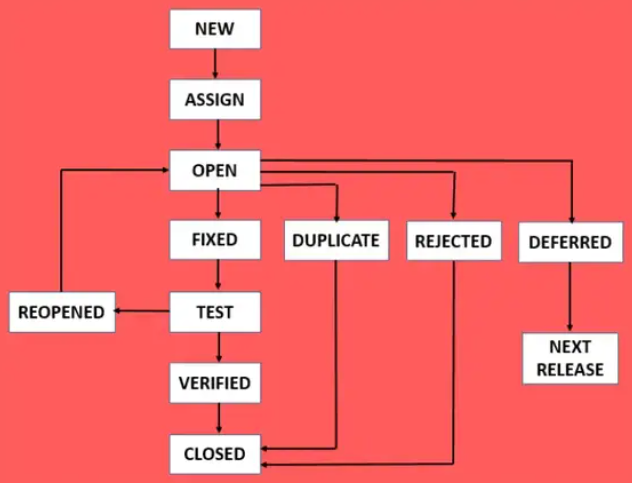
\includegraphics[width=0.6\textwidth]{bugLifecycle1.png}
    \attribution{https://www.softwaretestingmaterial.com/bug-life-cycle/}
\end{center}

\begin{itemize}
    \item Тестировщик выявил ошибку, она оказывается в статусе <<New>>.
    \item Тимлид, если счёл, что это реально ошибка, повесил ошибку на разработчика, она перешла в статус <<Assigned>>.
    \item Разработчик взялся за ошибку, перевёл её в состояние <<Open>>.
    \item Если такая ошибка (или другая, но с той же причиной) уже есть в трекере, ошибка переводится в состояние <<Duplicate>>.
    \item Если ошибка по мнению разработчика ошибкой не является, она переводится в статус <<Rejected>>.
    \item Если ошибка действительно ошибка, но пока нет ресурсов/смысла её править, она может отправиться в статус <<Deferred>> и в итоге перейти на следующий релиз (поменяв статус на <<Next Release>>).
    \item Самое интересное --- когда ошибку всё-таки исправили. Сначала разработчик выставляет её в статус <<Fixed>>, но на этом, конечно, её жизненный цикл не заканчивается.
    \item Тестировщик берёт поправленную ошибку на ретест, выставляя статус <<Test>>.
    \item Если ошибка не была поправлена (а по данным Канера, с первого раза нетривиальные ошибки удаётся поправить и ничего другого не сломать только в 20-50\% случаев), она отправляется в статус <<Reopened>> и снова к разработчику.
    \item Если была, то тестировщик переводит её в статус <<Verified>>.
    \item В конечном итоге, тимлид или тест-лид закрывает ошибку, отправляя её в статус <<Closed>>, где она пребывает до окончания проекта, чтобы потом можно было на неё ссылаться.
\end{itemize}

Вот более простая модель жизненного цикла ошибки, которая в целом даже чаще используется на практике:

\begin{center}
    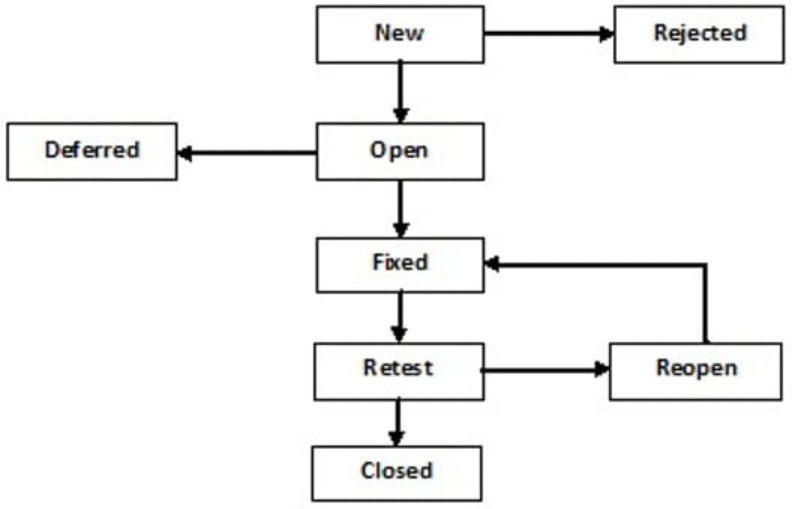
\includegraphics[width=0.6\textwidth]{bugLifecycle2.png}
    \attribution{https://www.softwaretestinghelp.com/bug-life-cycle/}
\end{center}

Или вот так жизненный цикл ошибки представляют себе начинающие тестировщики, однако на практике это не очень полезно:

\begin{center}
    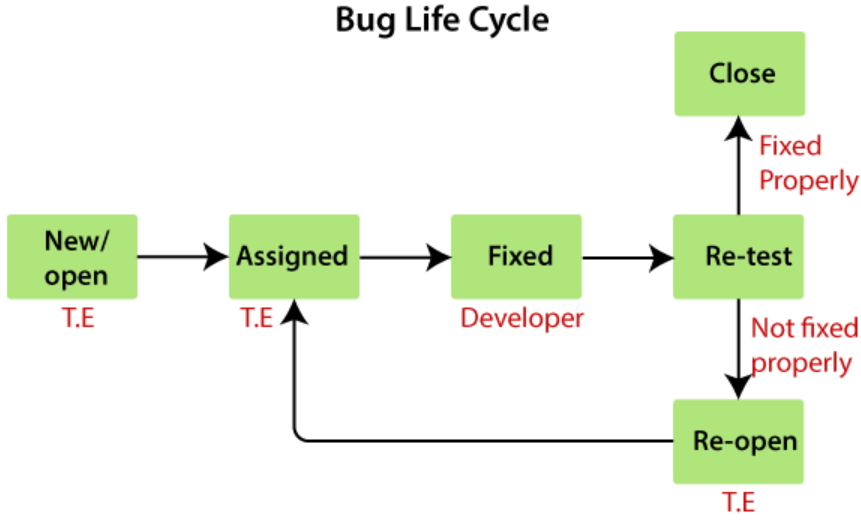
\includegraphics[width=0.6\textwidth]{bugLifecycle3.png}
    \attribution{https://www.javatpoint.com/software-testing-bug-life-cycle}
\end{center}

Но вообще, жизненный цикл ошибки подгоняется под практики конкретной команды, поэтому любая нормальная система управления ошибками должна уметь настраивать свой жизненный цикл.

\subsection{Системы отслеживания ошибок}

Среди реальных систем управления ошибками\footnote{Обратите внимание, это не то же, что системы управления тестовыми сценариями, а совсем другое.} стандартом де-факто является Atlassian Jira, которая на самом деле является полноценной системой управления проектами, а не только трекером дефектов, при этом очень настраиваема, имеет плагинную систему и кучу плагинов, однако платная. Поэтому у неё довольно много аналогов. 

В принципе, любая нормальная инфраструктура для разработки программного обеспечения умеет так или иначе отслеживать ошибки. Например, GitHub имеет очень неплохой, хоть и простой трекер GitHub Issues (например, в нём нет типов дефектов, не настраивается жизненный цикл, так что приходится всё это делать с помощью тэгов, которые он поддерживает), GitLab и подобные штуки тоже всё это умеют. Есть Yandex Tracker, Microsoft Team Foundation Server, Redmine (кстати, бесплатный, но что-то давно о нём не слышал в индустрии --- может, просто не попадался), JetBrains Youtrack. Для проектов с открытым исходным кодом также была популярна в своё время Bugzilla (как багтрекер, доступный конечным пользователям), но она старенькая и не очень удобная, поэтому её постепенно вытеснили конкуренты. Ещё инструменты управления проектами хороши для работы с ошибками, например, OpenProject (один из лучших таких инструментов с открытым исходным кодом).

\end{document}